\chapter{XÂY DỰNG MÔ HÌNH}

\label{Chapter3}
\section{Xây dựng mô hình}

\section{BLEU Score}
BLEU (BiLingual Evaluation Understudy) là một phương pháp sử dụng trong dịch máy (Machine translation). BLEU đánh giá một câu thông qua việc so sánh khớp giữa câu máy sinh ra (candidate) và câu mẫu (preference), giá trị của đánh giá từ khoảng 0 tới 1. Giá trị 0 thể hiện việc đầu ra sai hoàn toàn và giá trị 1 thể hiện việc đúng hoàn toàn. Thông thường giá trị BLEU đạt trên 40\% đã được coi là rất tốt \cite{lavie2010evaluating}.

BLEU đánh giá mô tả thông qua \cite{papineni2002bleu}:
\begin{itemize}
	\item Adequacy: Mô tả đầy đủ thông tin trong ảnh
	\item Fluency: Đúng ngữ pháp, cấu trúc câu
\end{itemize}

\begin{figure}[h!]
	\centering
	\subfigure{
		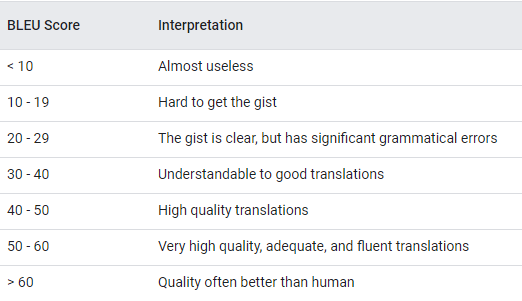
\includegraphics[width=14cm]{BLEU.png}}
	\subfigure{
		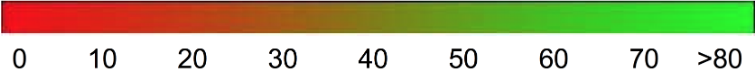
\includegraphics[width=14cm]{BLEU_scale.png}}         
	\caption{Đánh giá BLEU.}
\end{figure}

Đánh giá BLEU được tính toán như sau:
\begin{figure}[h!]
	\centering
	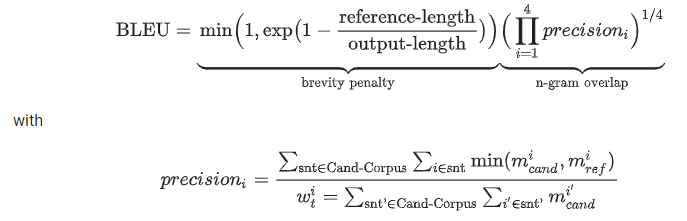
\includegraphics[width=15cm]{BLEU_cal.png}
	\caption{Tính toán đánh giá BLEU.}
\end{figure} 

Công thức tính bao gồm hai phần \cite{web:10}:
\begin{itemize}
	\item Brevity penalty:
	Dùng để hạn chế việc đánh giá tốt cho các câu ngắn và kém cho các câu dài hơn.
	\item N-gram overlap:
	Hoạt động như một hàm tính độ chính xác của đầu ra.
\end{itemize}

trong đó
\begin{itemize}
	\item $m_{cand}^i$: Số lượng i-gram trong candidate khớp với reference.
	\item $m_{ref}^i$: Số lượng i-gram trong reference.
	\item $w_{t}^i$: Tổng số i-gram trong candidate.
\end{itemize}
\section{Nhận xét kết quả}